% !TeX root = ../master.tex

\lecture{1}{2026-08-25}{Introduction to Heat Transfer}
These are the notes for the obligatory Heat Transfer course on the 5th semester of the Bs.c. in Mechanical Engineering at Aarhus University taught by Pourya Forooghi and Mugisa Y. Kano.

\section{Introduction to Heat Transfer}
Heat transfer as a subject has already been treated in the \href{https://www.bigum.dev/notes/partial-differential-equations.pdf}{Partial Differential Equations Course}.
Further, a related subject, namely \href{https://www.bigum.dev/notes/thermodynamics.pdf}{Thermodynamics} has also been studied.
However, whereas Thermodynamics mainly concerns itself with questions such as what the eventual equilibrium temperature will be or the total amount of heat transferred, heat transfer as a subject is more interested in questions such as the time it takes or the rate of heat transfer.

Heat Transfer is used in both power generation, heating/cooling/refrigeration, the chemical industry, indoor climate, thermal management and much more.
Further, new technology means heat transfer will remain very useful into the future as data centers, electronics, and turbine blades all need to meet higher cooling standards to maintain performance. 

Before we start, a quick note on terminology is useful.
We distinguish between \textit{Heat}, \textit{Heat transfer rate}, and \textit{Heat flux}.
Heat, $Q [\unit{\J}]$, denotes the amount of heat transfered.
The heat transfer rate, $\dot{Q}, [\unit{\J\per\s}]$, denotes the heat $Q$ transferred per unit time.
And finally, Heat flux, $\dot{q} [\unit{\W\per\m\squared}]$, is the heat transfer rate $\dot{Q}$ per unit area.

\subsection{Thermodynamics Recap}
Here will be given a short Introduction to the most important concepts of Thermodynamics which we will be dealing with here.
For a more in-depth review of the material see \href{https://www.bigum.dev/notes/thermodynamics.pdf}{my notes on the subject}.

The change in internal energy $u$ and enthalpy $h=u+p / \rho$ with temperature is generally given as:
\begin{itemize}
  \item Ideal Gasses:
    \begin{align*}
      \mathrm{d}u &= c_v \, \mathrm{d}T \\
      \mathrm{d}h = c_p \, \mathrm{d}T
    .\end{align*}
  \item Incompressible substances:
    \begin{equation*}
      \mathrm{d}u = c \, \mathrm{d}T \quad (c \approx c_p \approx c_v)
    .\end{equation*}
\end{itemize}

Also, the 1st law of thermodynamics (the energy balance) states that the net energy transfer by heat, work, and mass from a system equals the change in the total energy of said system.
This also implies that the rate of energy transfer equals the rate of change in total energy.

\section{Heat Transfer Mechanisms}
We mainly work with three different heat transfer mechanisms.
These are \textit{Conduction}, \textit{Convection}, and \textit{Radiation}.

\subsection{Conduction}
\begin{wrapfigure}{r}{0.4\textwidth}
  \vspace{-1.5cm}
  \centering
  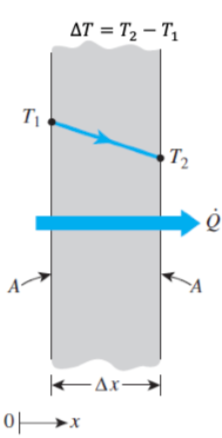
\includegraphics[width=\linewidth]{./figures/conduction.png}
  \caption{Cross section of a material displaying thermal conduction \citepage{cengel2015heatmasstransfer}{fig.~1--23}.}
  \label{fig:conduction}
\end{wrapfigure}
Conduction is the transfer of energy from more energetic particles of a substance to the adjacent less energetic ones.
This happens in both solids and fluids, but always through a material medium, so it cannot happen in a vacuum.

The rate of conduction $\dot{Q}_{\mathrm{cond}}$ is generally given on a form resembling:
\begin{equation*}
  \dot{Q}_{\mathrm{cond}} \propto A \frac{\Delta T}{\Delta x}
\end{equation*}
where $A$ is the conducting area, $\Delta T$ is the change in temperature and $\Delta x$is the thickness of the cross-section.
This can be qualified by including the \textit{thermal conductivity} $\left[ \unit{\W\per\m\per\K} \right]$ which gives:
\begin{equation*}
  \dot{Q}_{\mathrm{cond}} = -k A \frac{\Delta T}{\Delta x}
.\end{equation*}
As $\Delta x \to 0$ this turns into \textit{Fourier's law of conduction (1D)}, given as:
\begin{equation*}
  \dot{q}_{\mathrm{cond}} = -k \frac{\mathrm{d}T}{\mathrm{d}x} 
\end{equation*}
or in general vector form as 
\begin{equation*}
  \Vec{\dot{q}} = -k \nabla T
.\end{equation*}
The thermal conductivity is a material property which varies with temperature.

We also define the \textit{thermal diffusivity} $\alpha$ as
\begin{equation*}
  \alpha = \frac{k}{\rho c_p}
.\end{equation*}
Roughly speaking, the thermal diffusivity determines how fast heat diffuses in a certain solid material.

\subsection{Convection}
\begin{wrapfigure}{r}{0.35\textwidth}
  \vspace{-1.5cm}
  \centering
  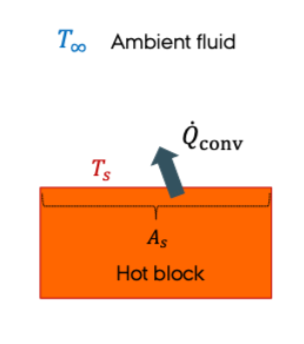
\includegraphics[width=\linewidth]{./figures/convection.png}
  \caption{Cross section of a material displaying convection.}
  \label{fig:conduction}
\end{wrapfigure}
Convection is the transfer of energy as a result of bulk motion of fluid.
This always happens between a solid surface and a flowing fluid.
This can be both \textit{natural (free) convection}, i.e. flow created by bouyancy force and \textit{forced convection}, i.e. flow created by an external driving force.
When a material undergoes convection it will generally also be undergoing convection to some degree. 

The convection rate $\dot{Q}_{\mathrm{conv}}$ is normally given in a form such as
\begin{equation*}
  \dot{Q}_{conv} = \propto A_s (T_s - T_{\infty})
\end{equation*}
where $T_{\infty}$ is the far field temperature (or some other reference temperature), $T_s$ is the surface temperature, and $A_s$ is the heat transfer surface area. 
By introducing the heat transfer coefficient $h \left[ \unit{\W\per\m\squared\per\K}  \right]$ we arrive at Newton's law of cooling:
\begin{equation*}
  \dot{Q}_{\mathrm{conv}} = h A_s \left( T_s - T_{\infty} \right)
.\end{equation*}
It is important to remember the difference between the thermal conductivity $k$ and the heat transfer coefficient $h$.
Whereas the thermal conductivity is a material property the heat transfer coefficient is a property of the specific flow and must therefore be experimentally determined in all but the simplest cases.

\subsection{Radiation}
Thermal radiation is energy emitted by matter in form of electromagnetic waves.
Here, there is no need for an intervening medium, so this may also happen in a vacuum.
All bodies at a temperature above \qty{0}{\K} emit thermal radiation.
In general, radiation is a volumetric phenomenon but for opaque solids it is usually considered a surface phenomenon.
The heat transfer rate due to radiation, $\dot{Q}_{\mathrm{emit}}$:
\begin{equation*}
  \dot{Q}_{\mathrm{emit}} \propto A_s T_s^{4}
.\end{equation*}
For a black body (an ideal radiator) this is preciselu:
\begin{equation*}
  \dot{Q}_{\mathrm{emit}} = \sigma A_s T_s^{4}
\end{equation*}
where $\sigma = \qty{5,670e-8}{\W\per\m\squared\per\K^{4}}$ is Boltzmann's constant. The above is also known as Boltzmann's law.
For an arbitrary surface we instead have
\begin{equation*}
  \dot{Q}_{\mathrm{emit}} = \epsilon \sigma A_s T_s^{4}
\end{equation*}
where $0 \leq \epsilon \leq 1$ is the emissivity. 

Emissivity $\epsilon$ is a property of the radiating surface, which in reality varies with temperature but also depends on the wavelength of the electromagnetic wave.
For simplicity, we often use its mean value.

The opposite case of emitted radiation is that of absorbed radiation given by
\begin{equation*}
  \dot{Q}_{\mathrm{abs}} = \alpha \dot{Q}_{\mathrm{incident}}
\end{equation*}
where $0 \leq \alpha \leq 1$ is the absorptivity. 
Kirchoff's law of radiation states that at the same temperature and wavelength $\epsilon = \alpha$.

The net radiation heat transfer of a solid surface is
\begin{equation*}
  \dot{Q}_{\mathrm{rad}} = \dot{Q}_{\mathrm{emit}} - \dot{Q}_{abs}
.\end{equation*}
We have an important special case of the above for a surface entirely enclosed by a much larger surrounding surface as shown on \Cref{fig:radiation}, where
\begin{equation*}
  \dot{Q}_{\mathrm{rad}} = \epsilon \sigma A_s \left( T_s^{4} - T^{4}_{\mathrm{surr}} \right)
.\end{equation*}


\begin{figure} [ht]
  \centering
  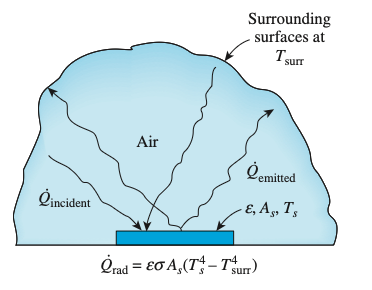
\includegraphics[width=0.5\linewidth]{./figures/radiation.png}
  \caption{Radiation between enclosed and enclosing body\citepage{cengel2015heatmasstransfer}{fig.~1--40}.}
  \label{fig:radiation}
\end{figure}
